%template1.tex
%The following LaTeX source file represents the simplest kind of slide presentation; no overlays, no included graphics. Substitute your favorite style for ``pascal''. To create the PDF file template1.pdf, (1) be sure to use the prosper class, then (2) execute the command latex template1.tex, and (3) the command dvipdf template1.dvi.

%%%%%%%%%%%%%%%%%%%%%%%%%%%%%%% template1.tex %%%%%%%%%%%%%%%%%%%%%%%%%%%%%%%%%%%
\documentclass[a4paper,blends,pdf,colorBG,slideColor]{prosper}
% definitions for slides for CSC544
% Lutz Hamel, (c) 2007

\hypersetup{pdfpagemode=FullScreen}

\usepackage{times}
\usepackage{latexsym}
\usepackage{alltt}
\usepackage{booktabs}
\usepackage{amsmath}
\usepackage{amsopn}
\usepackage{amsfonts}
\usepackage{amssymb}
%\usepackage[usenames]{color}

\def\sign{\qopname\relax{no}{sign}}
\def\argmax{\qopname\relax{no}{argmax}}
\def\argmin{\qopname\relax{no}{argmin}}

\newcommand{\grad}{\ensuremath{\nabla}} 
\newcommand{\loss}{\ensuremath{{\cal L}}}
\newcommand{\err}{\mbox{err}}
\newcommand{\mse}{\mbox{mse}}
\newcommand{\acc}{\mbox{acc}}
\newcommand{\Integer}{\ensuremath{\mathbb{N}}}
\newcommand{\size}[1]{{|{#1}|}}
\newcommand{\Rnspace}[1]{\ensuremath{\mathbb{R}^{#1}}}
\newcommand{\Real}{\ensuremath{\mathbb{R}}}
\newcommand{\mytt}[1]{{\small\tt{#1}}}
\newcommand{\textemph}[1]{{\em #1}}
\newcommand{\suchthat}{\mid}
\newcommand{\orbar}{\;|\;}
\newcommand{\bs}[1]{\begin{slide}{#1}\ptsize{8}}
\newcommand{\es}{\end{slide}}
\newcommand{\co}{\,\colon\;}
\newcommand{\pair}[2]{\ensuremath{( {#1}, {#2} )}}
\newcommand{\model}[1]{\hat{#1}}
\newcommand{\ul}[1]{{\bf\em #1}}
\newcommand{\ol}{\overline}
\newcommand{\definition}[1]{{\bf Definition: }{\em #1}}
\newcommand{\example}[1]{{\bf Example: }{#1}}
\newcommand{\abs}[1]{|{#1}|}
\newcommand{\mytab}{\makebox[.1in]{}}

\newcommand{\fdef}[1]{
\begin{center}
\fbox{
\begin{minipage}{3.5in}
{\bf Definition:}
{#1}
\end{minipage}
}
\end{center}
}

\newcommand{\fframe}[1]{
\begin{center}
\fbox{
\begin{minipage}{3.5in}
{#1}
\end{minipage}
}
\end{center}
}

\newcommand{\nframe}[1]{
\begin{center}
\begin{minipage}{3.5in}
{#1}
\end{minipage}
\end{center}
}

\newenvironment{Rcode}
	{
		\scriptsize
		\begin{quote}
		\begin{alltt}
	}
	{
		\end{alltt}
		\end{quote}
	}




\begin{document}
\bs{Statistical Computing in R}
R is a programming language designed to support data analysis and model building.

\begin{itemize}
\item All traditional programming constructs such as expressions, assignments, conditionals, loops, and functions are present.
\item A straight-forward object system that supports high-level constructs such as statistical models with all their parameters etc. very nicely.
\item Vector arithmetic (very powerful and the preferred way of accomplishing things in R).
\item Graphics engine supporting graphical techniques (automatic scatter plots, histograms, etc.)
\item Many, many extension modules implementing everything from basic statistics to micro array analysis...and in particular support vector machines.
\end{itemize}
\es

\bs{Interactive R Session}
\begin{center}
   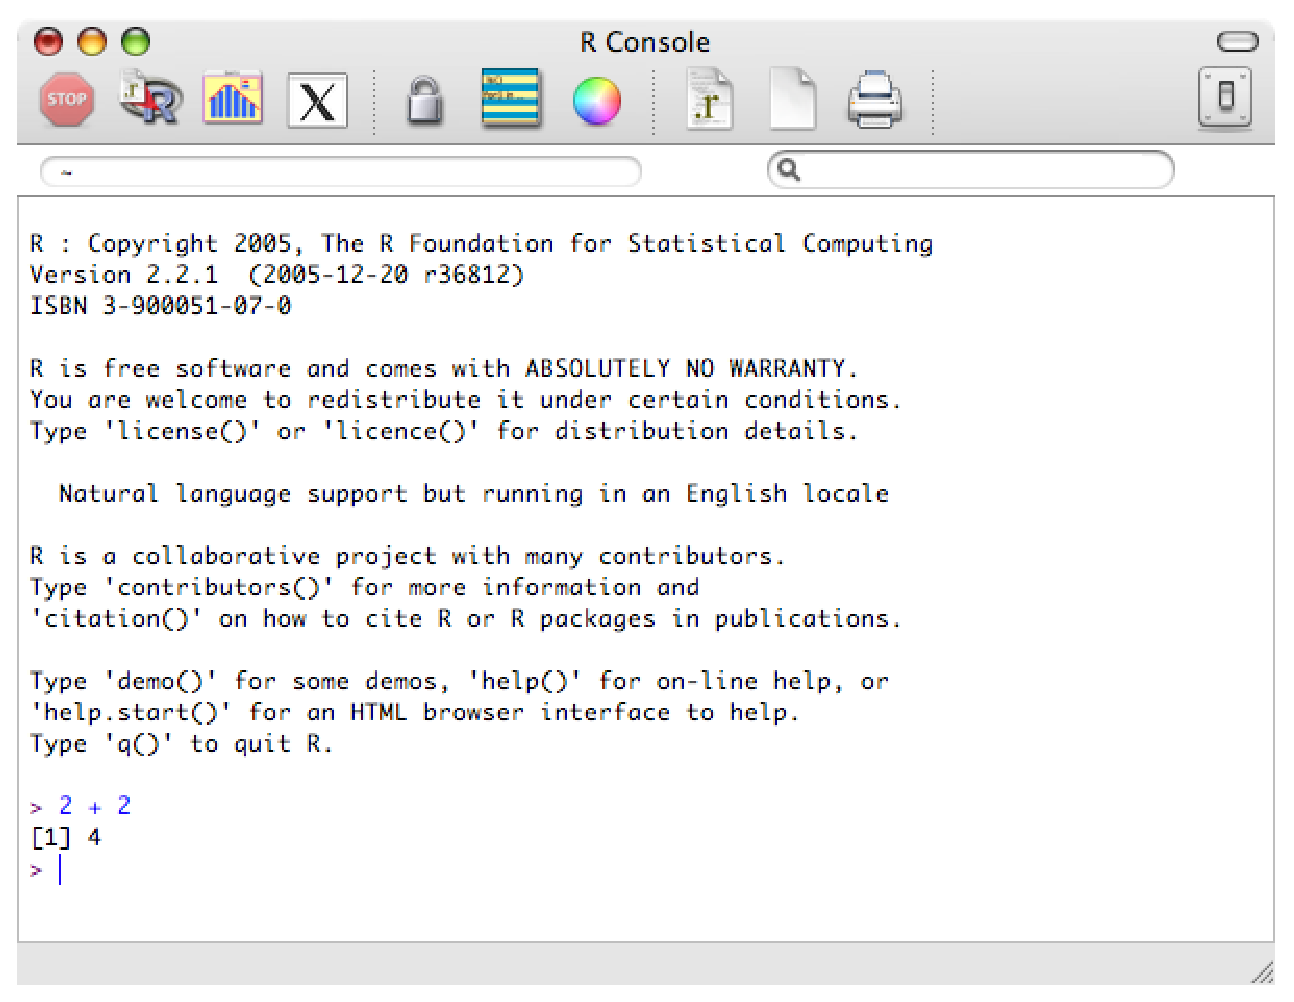
\includegraphics[height=60mm]{figures/r-screen.eps}
\end{center}
\es

\bs{R Programming}
\begin{minipage}[t]{1in}
\begin{verbatim}
> x <- 2
> 2 * x
[1] 4
\end{verbatim}
\end{minipage}
\begin{minipage}[t]{1.5in}
\begin{verbatim}
> v <- c(1,2,3)
> v
[1] 1 2 3
\end{verbatim}
\end{minipage}
\begin{minipage}[t]{1in}
\begin{verbatim}
> v + 1
[1] 2 3 4
\end{verbatim}
\end{minipage}

\vspace{.5in}

\begin{minipage}[t]{1.5in}
\begin{verbatim}
> w <- v + 1
> q <- w + v
> q
[1] 3 5 7
\end{verbatim}
\end{minipage}
\begin{minipage}[t]{2in}
\begin{verbatim}
> add1 <- function(x) { x + 1; }
> add1
function(x) { x + 1; }
> add1(1)
[1] 2
\end{verbatim}
\end{minipage}

\es

\bs{R Programming}
\begin{minipage}[t]{2in}
\begin{verbatim}
> addv1
function(v) 
   { 
      y <- c() 
      for (x in v) { 
         x1 <- x + 1 
         y <- c(y,x1)
      } 
      y
   }
> w
[1] 2 3 4
> addv1(w)
[1] 3 4 5
\end{verbatim}
\end{minipage}
\begin{minipage}[t]{2in}
This function performs the same operation as the vector operation {\tt w  + 1}.
From a performance point of view it is always desirable to use the vector operations,
explicit iteration over vector elements is SLOW!
\end{minipage}

\es

\bs{R Data}
R has many different ways to represent data:
\begin{itemize}
\item vectors
\item lists
\item arrays/matrices
\end{itemize}
The most important one (for our purposes) is the {\em data frame}.  A data frame is
a two-dimensional data matrix with additional structure.
\begin{center}
\begin{minipage}[t]{2in}
\begin{verbatim}
> df <- data.frame(v,w)
> df
  v w
1 1 2
2 2 3
3 3 4
> df$v
[1] 1 2 3
> df$w
[1] 2 3 4
\end{verbatim}
\end{minipage}
\end{center}
\es

\bs{Loading Data Frames}
We can read comma-separated-value (CSV) files directly into an R data frame.

Here is our mammal training data set represented as a CSV file:

\begin{Rcode}
Legs, Wings, Fur, Feathers, Mammal
4, no, yes, no, true
2, yes, no, yes, false
4, no, no, no, false
4, yes, yes, no, true
3, no, no, no, false
\end{Rcode}

Assume that we saved this into a file called ``mammals.csv'', in a directory called ``datasets''.
\es

\bs{Loading Data Frames}
 \begin{Rcode}
> setwd("datasets")
> mammals.df <- read.csv("mammals.csv")
> mammals.df
  Legs Wings  Fur Feathers Mammal
1    4    no  yes       no   true
2    2   yes   no      yes  false
3    4    no   no       no  false
4    4   yes  yes       no   true
5    3    no   no       no  false
> summary(mammals.df)
      Legs      Wings     Fur    Feathers    Mammal 
 Min.   :2.0    no :3    no :3    no :4    false:3  
 1st Qu.:3.0    yes:2    yes:2    yes:1    true :2  
 Median :4.0                                        
 Mean   :3.4                                        
 3rd Qu.:4.0                                        
 Max.   :4.0                                        
 \end{Rcode}
\es

\bs{R Built-in Data Frames}
For convenience sake, R comes with a number of predefined data frames.  One such
predefined data frame is the {\em iris data set}.
{\scriptsize
\begin{center}
\begin{minipage}[t]{5in}
\begin{verbatim}
> data(iris)
> summary(iris)
  Sepal.Length    Sepal.Width     Petal.Length    Petal.Width          Species  
 Min.   :4.300   Min.   :2.000   Min.   :1.000   Min.   :0.100   setosa    :50  
 1st Qu.:5.100   1st Qu.:2.800   1st Qu.:1.600   1st Qu.:0.300   versicolor:50  
 Median :5.800   Median :3.000   Median :4.350   Median :1.300   virginica :50  
 Mean   :5.843   Mean   :3.057   Mean   :3.758   Mean   :1.199                  
 3rd Qu.:6.400   3rd Qu.:3.300   3rd Qu.:5.100   3rd Qu.:1.800                  
 Max.   :7.900   Max.   :4.400   Max.   :6.900   Max.   :2.500    
\end{verbatim}
\end{minipage}
\end{center}
}

\vspace{.2in}
We might wish to inspect the data distributions visually as well:
\begin{verbatim}
> hist(iris$Sepal.Length)
> hist(iris$Petal.Length)
\end{verbatim}
\es

\bs{R Built-in Data Frames}
\begin{center}
   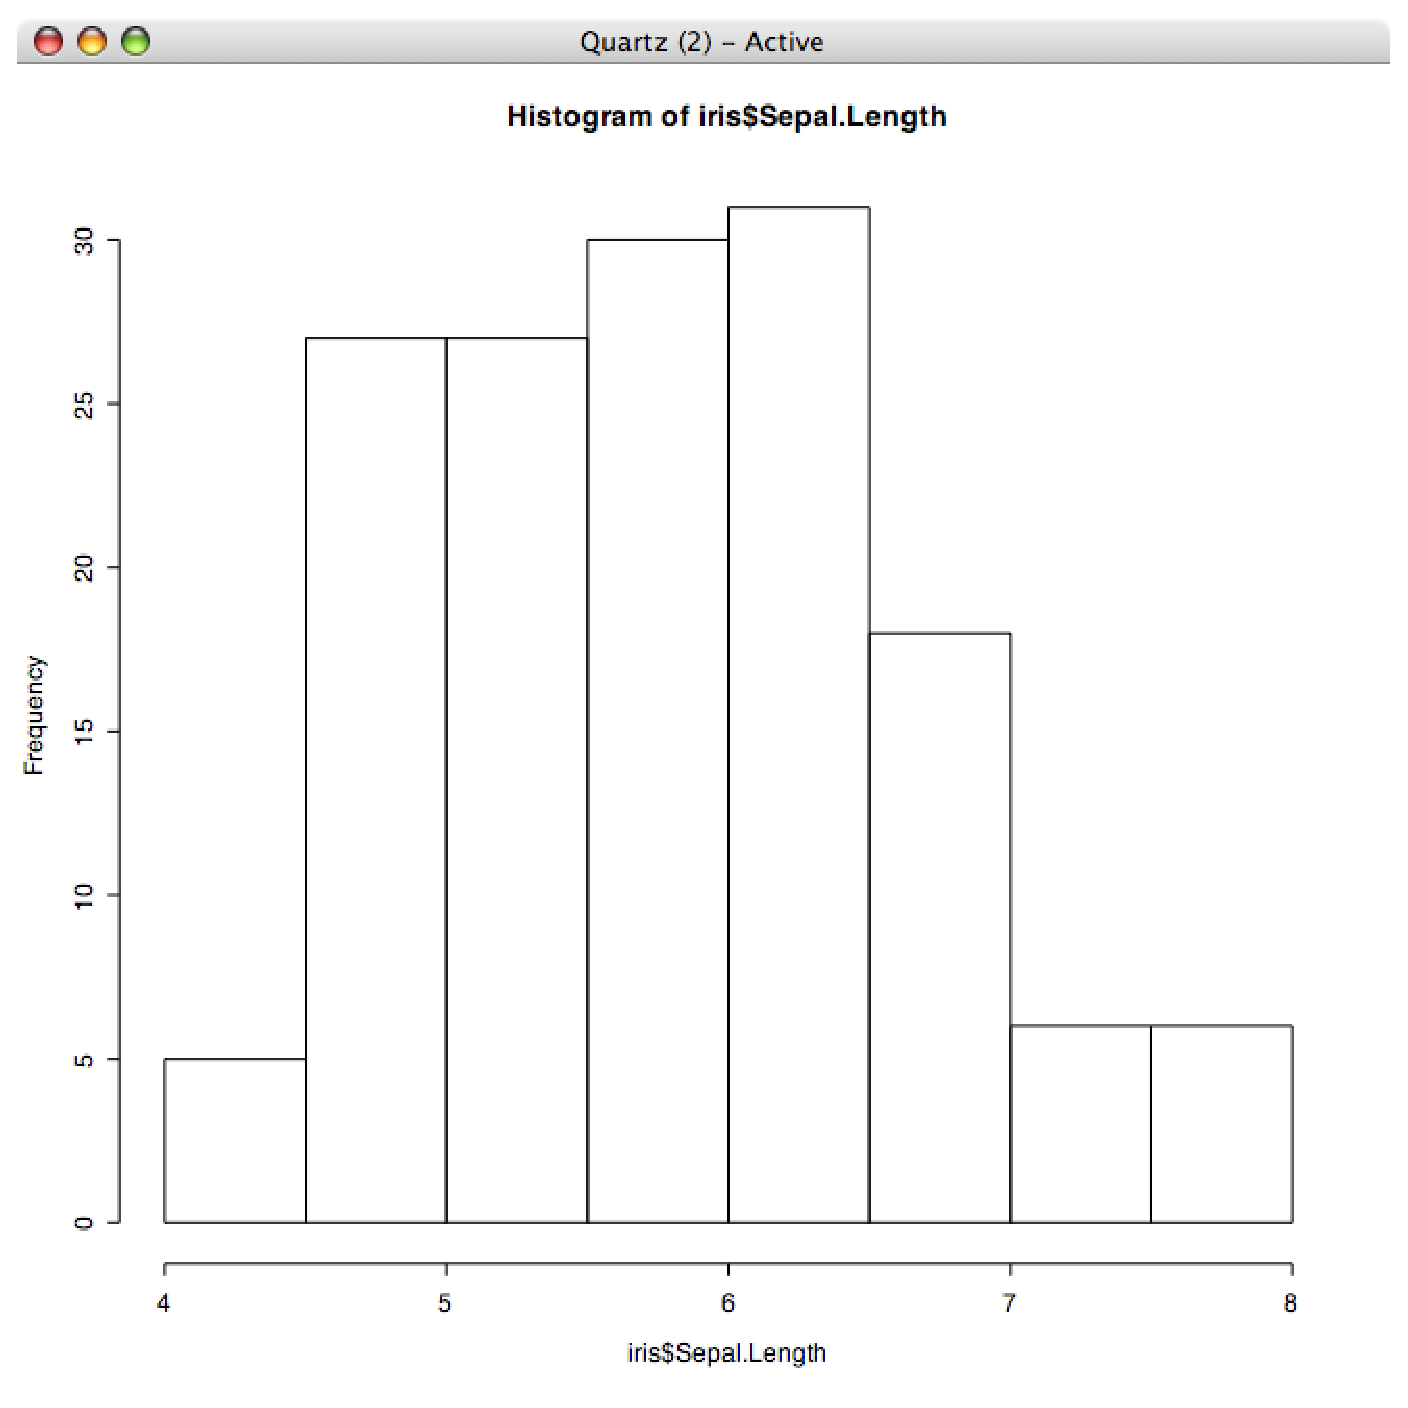
\includegraphics[height=50mm]{figures/sepal-length.eps}
   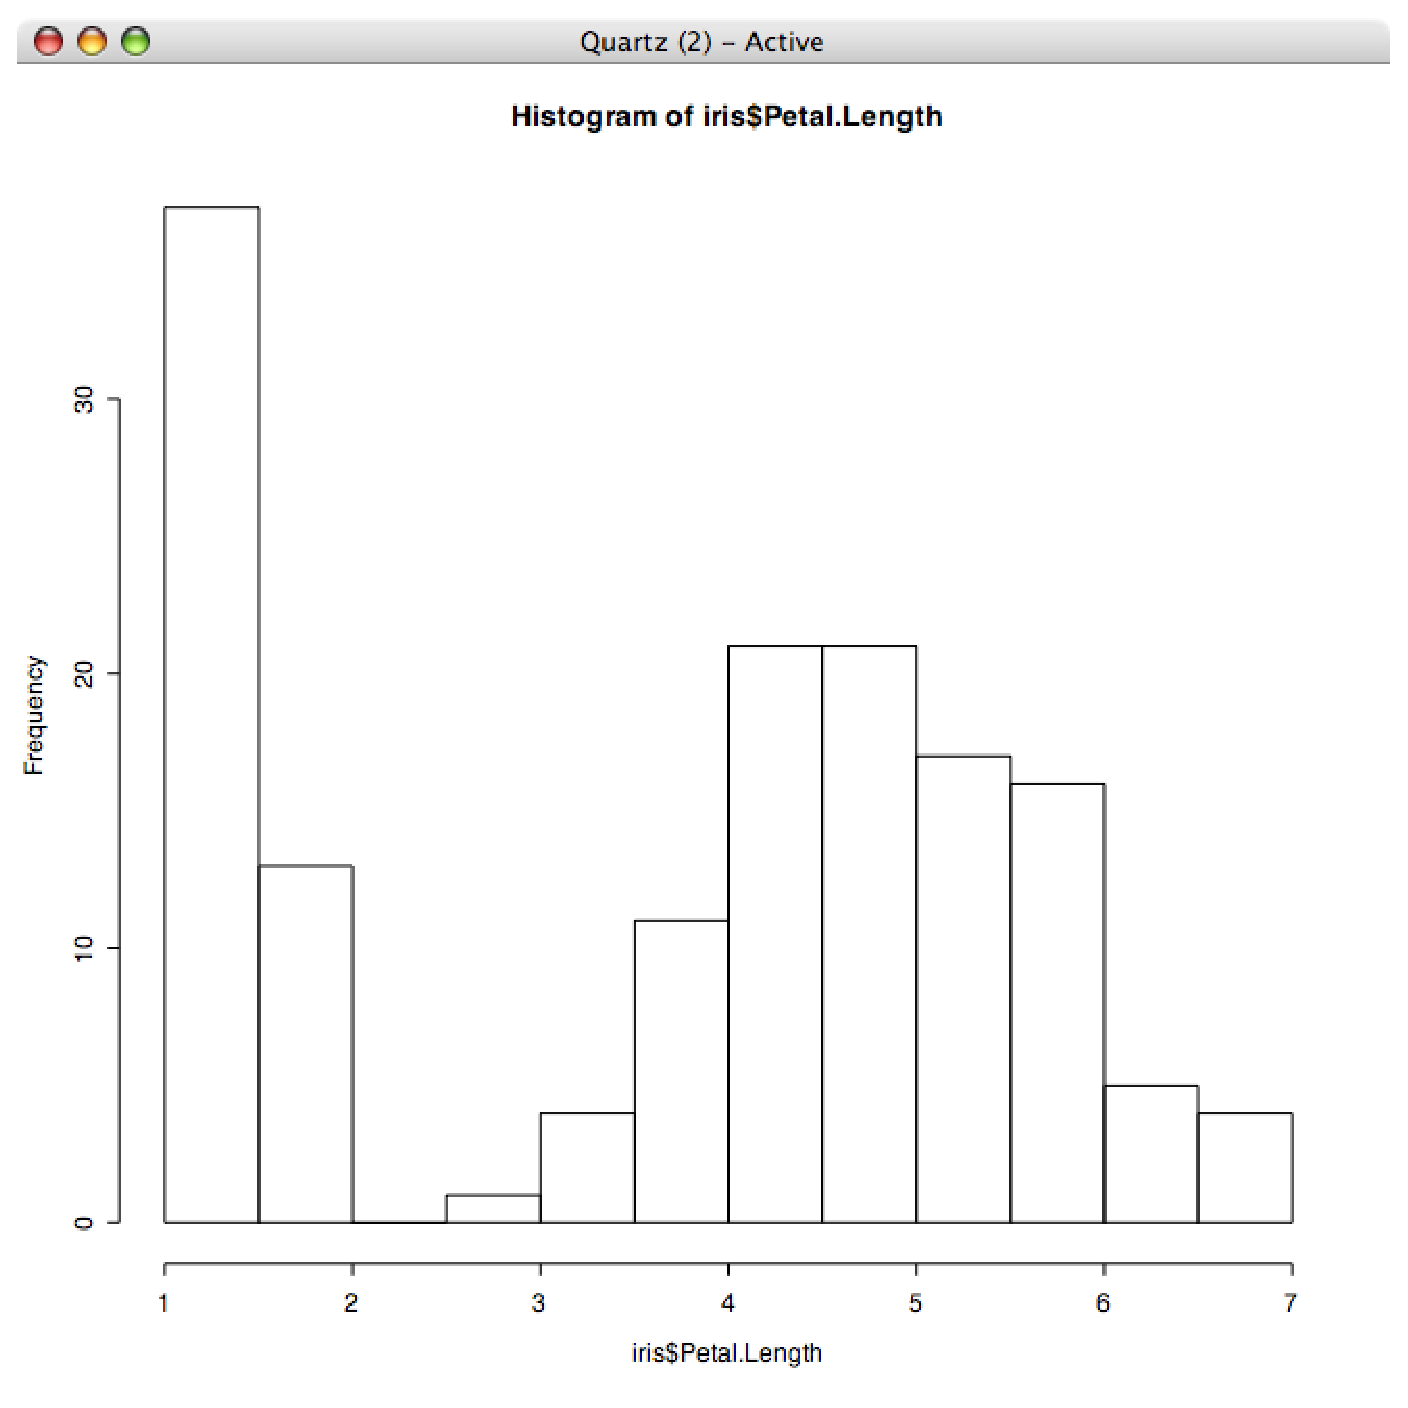
\includegraphics[height=50mm]{figures/petal-length.eps}
\end{center}
\es

\bs{R Built-in Data Frames}
\begin{verbatim}
> plot(iris)
\end{verbatim}
\begin{center}
   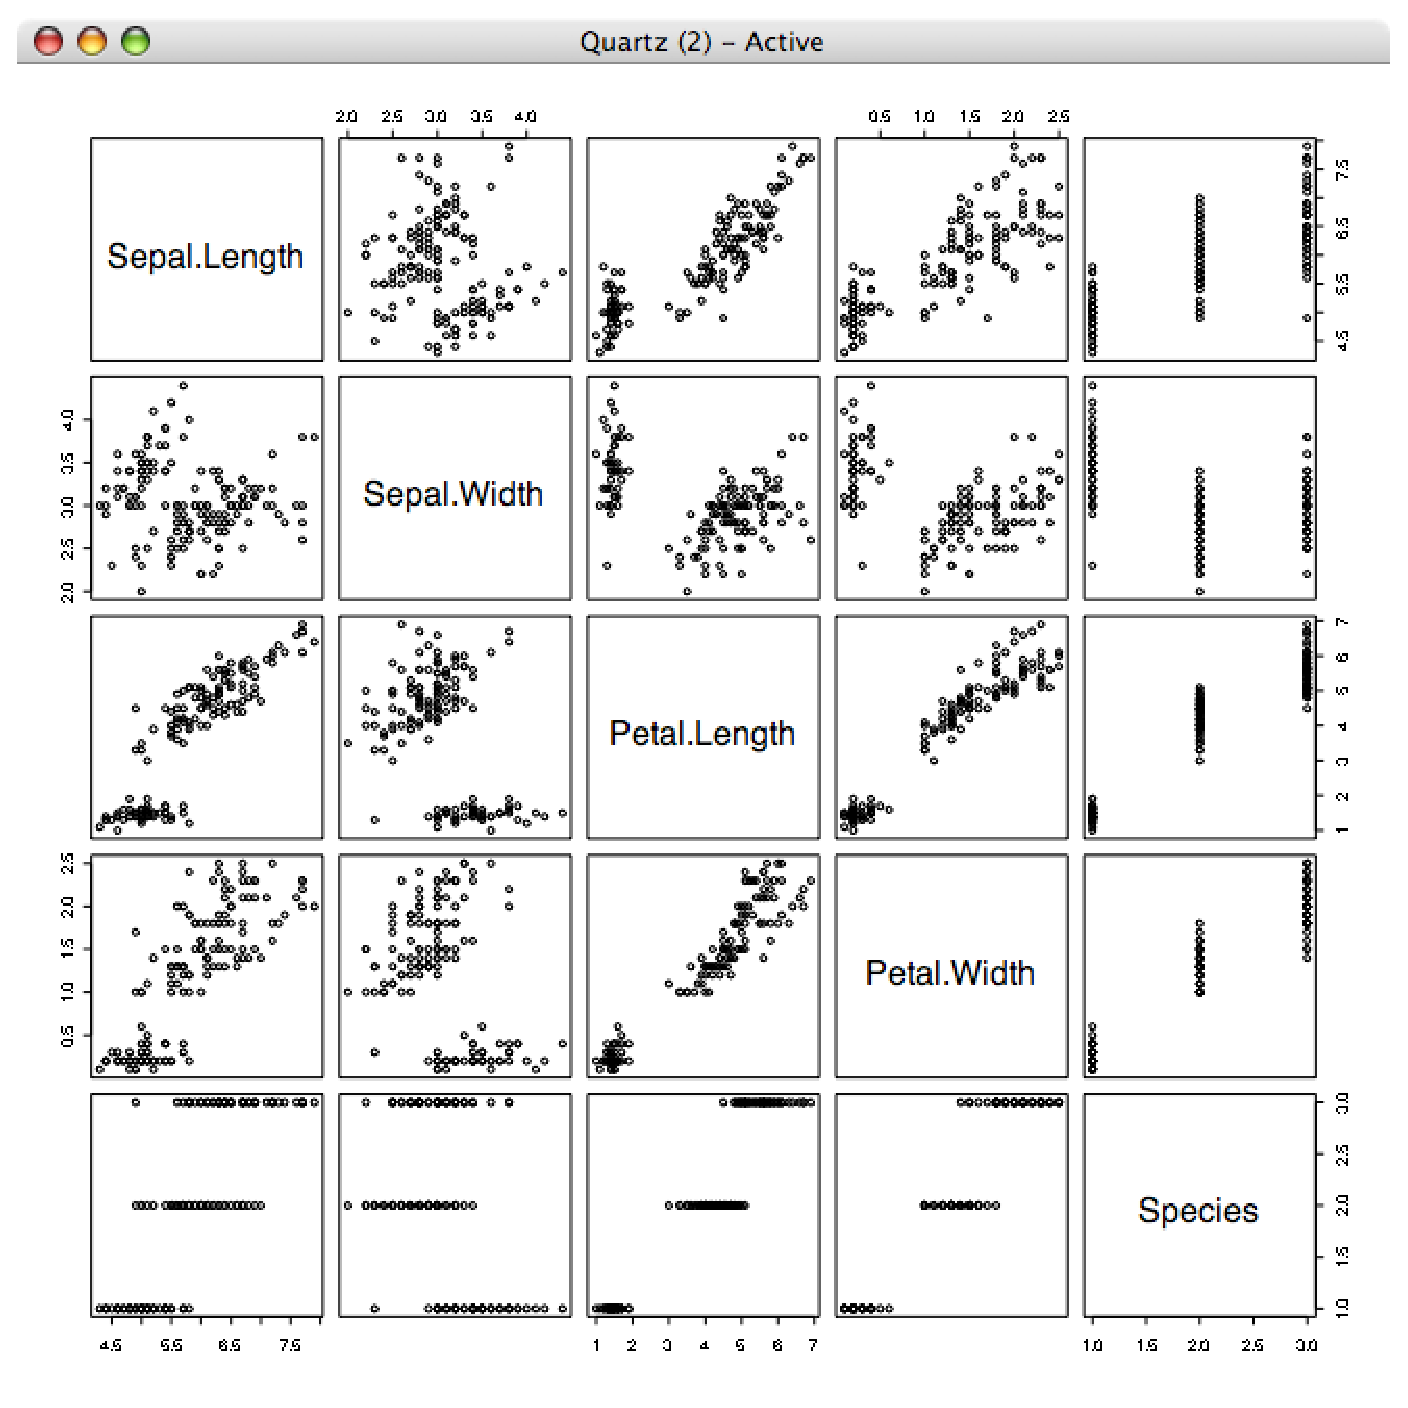
\includegraphics[height=60mm]{figures/iris-scatter.eps}
\end{center}
\es

\bs{Simple Model Building}
{\scriptsize
\begin{verbatim}
> attach(iris)
> model <- lm(Petal.Length~Petal.Width)
> plot(Petal.Width,Petal.Length)
> abline(model)
\end{verbatim}
}
\begin{center}
   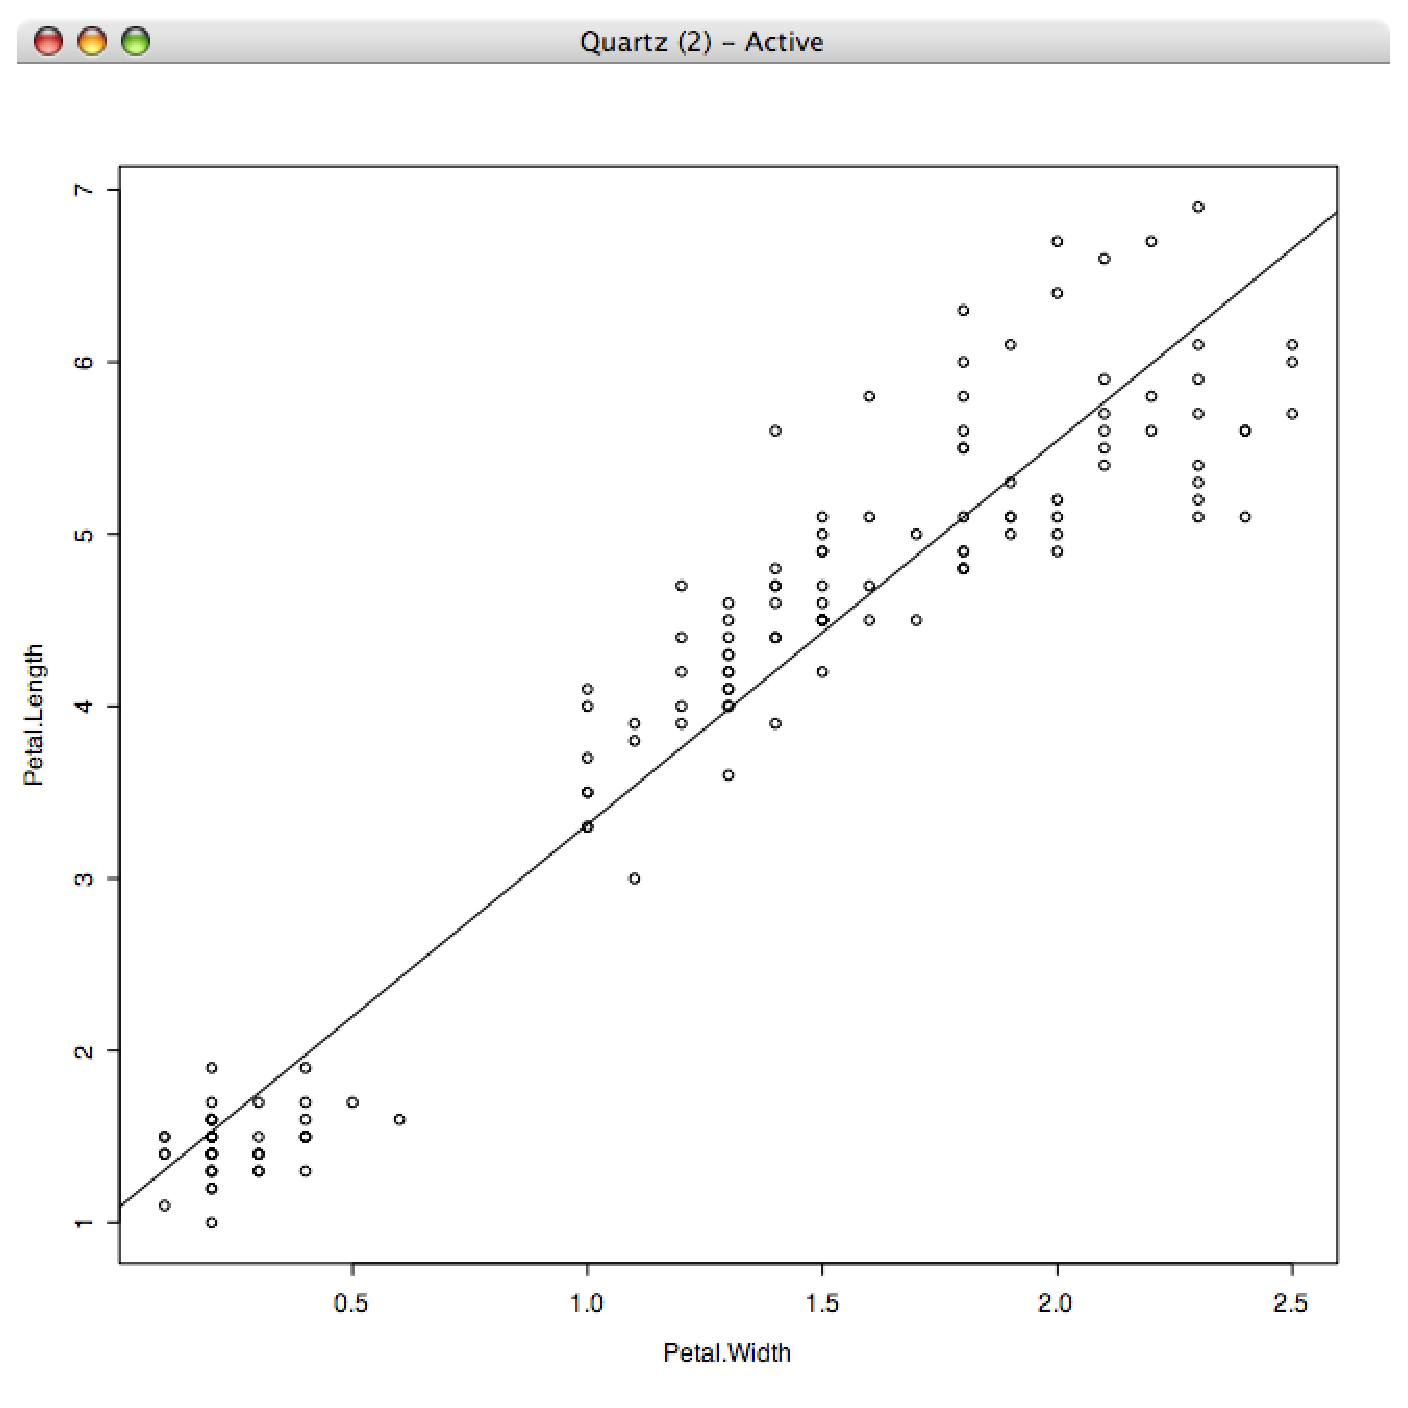
\includegraphics[height=60mm]{figures/iris-model.eps}
\end{center}

\es

\bs{Homework}
Read Chapter 1 and Appendix B

Do Assignment 1, see website.
\es

\end{document}
%%%%%%%%%%%%%%%%%%%%%%%%%%% end of template1.tex %%%%%%%%%%%%%%%%%%%%%%%%%%%%%%%%

